\chapter{Dynamic models and Bayesian inference}\label{ch:dynamics}

A reader who arrives at this chapter from the physical sciences brings a belief that deserves
a fair hearing. The borrowers in a credit register do not sit still. Their exposures grow
and shrink, their loans start and end, and the cells of a release table fill and empty as the
months pass. Physics has spent two centuries writing equations for quantities that move,
and the best of them, the conservation laws and the Navier--Stokes equations of fluid flow,
are among the most tested statements in science. On this view a model drawn from physics,
with more equations and more structure, must forecast disclosure risk better than the counts
and tables used in the rest of this book. The structure carries knowledge that the data alone
cannot supply: mass is not created from nothing, densities do not go negative, change is
smooth. A risk forecast that respects these rules ought to be more accurate than one that
does not.

The first fact that breaks the belief is a fact about this book's own evidence. No transport model in this book has yet beaten a simpler baseline on held-out data, because that
comparison has not been run. The claim ledger records the idea that Navier--Stokes
describes the movement of information as a proposed analogy, unestablished, and it records
the general Navier--Stokes solver as not built, conditional on a simpler model being shown
to fall short. A second fact comes from the one experiment that was run. When the equations were fitted to observations that they had generated themselves, with the parameters
known in advance, the observations responded about fourteen times more strongly to one
parameter than to the other, in the units the model uses, and the weaker one was the drift
that the model exists to forecast. Structure in a model is a set of assumptions. It helps a
forecast only where the assumptions are true and the data can resolve the parameters they
introduce, and both of those are things to be shown.

This chapter asks one question. What would a dynamic model of the target population
have to show before its forecast could enter a release decision? The answer is built in layers:
what such a model can mean for disclosure, how its equations are solved and checked, how
its parameters are inferred from data and how far the data can identify them, and which
simpler model it has to beat.

\section{A proposal from a visiting researcher}

Tom\'as, the visiting researcher whose requests for credit-register files run through earlier
chapters, came to Naledi with a different kind of proposal. He had trained in applied mathematics before turning to finance, and he wanted to model how the Bank's borrowers drift
across the space of exposure and lending relationships from one vintage to the next. If the
drift could be forecast, he argued, the Bank could see in advance which cells of a release
table were thinning out and becoming risky, and set its floors before the risk arrived. His
note proposed an advection--diffusion equation for the density of borrowers, with a drift
field governed by the Navier--Stokes equations.

Naledi read the note twice before replying. She did not doubt the mathematics. Her
question was what each symbol stood for in the register, and what evidence would tell the
committee that the forecast was better than the one it already had. She asked Tom\'as to
answer both in writing before the proposal went any further.

\section{What a fluid equation can and cannot mean here}

The Navier--Stokes equations describe the balance of momentum in a fluid. A credit register
has no mass of information, no momentum and no pressure law, and an analogy does not
supply them. What the equations can offer is narrower: a declared regularisation model
for how a population moves across a space of features. Such a model may help to generate
coherent stress scenarios or to smooth a distribution that changes over time. Whether it forecasts disclosure risk better than a simpler model is an empirical question, and this chapter
treats it as one.

The space must be built with care. Let $x\in\Omega$ be a feature vector made from continuous
quantities, such as standardised log exposure and a continuous measure of how concentrated a borrower's lending relationships are. Integer codes for sectors, regions or lenders
do not define a distance; sector 4 is not closer to sector 5 than to sector 12. Categorical relationships belong in a graph or in separate strata, as Section~\ref{c20:sec-baseline} sets out. An embedding
that turns categories into coordinates must be fitted on development data, frozen, and tested
for distortion, because a rotation or rescaling of the embedding would otherwise change the
scientific claim without anyone deciding to change it.

On that space let $c(x,t)\ge0$ be the density of target states at time $t$. It is a population
distribution: it says where the borrowers are, not how exposed they are. Let $u(x,t)$ be the
drift of features, $D_c>0$ a dispersion coefficient and $s(x,t)$ the net rate at which targets enter
or leave. For any fixed region $V\subset\Omega$ with outward normal $n$, the mass in $V$ changes only
by flux through its boundary and by entry and exit:
\begin{equation}\label{c20:eq-balance}
\frac{d}{dt}\int_V c\,dx=-\int_{\partial V}(c\,u-D_c\nabla c)\cdot n\,dS+\int_V s\,dx.
\end{equation}
Because $V$ is arbitrary, the divergence theorem turns this into the advection--diffusion equation
\begin{equation}\label{c20:eq-ad}
\partial_t c+\nabla\!\cdot(c\,u)=D_c\Delta c+s.
\end{equation}
With periodic boundaries, or boundaries that let no mass through, and with $s=0$, the total
mass $\int_\Omega c\,dx$ is constant. With entry and exit it changes by $\int_\Omega s\,dx$ per unit time. A density
that does not satisfy this balance should not be normalised and then read as a probability.
Resetting the total to one after every numerical step is a common shortcut, and it hides
exactly the conservation error that the balance is there to catch; if normalisation is needed,
the equation for the normalised density should be derived.

The density is not yet a risk. The link to the disclosure experiment of Chapter~2 comes
through an attack response $g_a(x,\theta)\in[0,1]$, the probability that attack $a$ names the right
record for a target with features $x$ when the release uses protection setting $\theta$. The model
risk is the average response over the population:
\begin{equation}\label{c20:eq-risk}
r_a(\theta,t)=\frac{\int_\Omega g_a(x,\theta)\,c(x,t)\,dx}{\int_\Omega c(x,t)\,dx}.
\end{equation}
Everything a dynamic model says about disclosure passes through $g_a$, and $g_a$ must be fitted
to measured attack outcomes, the counts of Chapter~\ref{ch:estimate}. A density that moves without a fitted
response says nothing about disclosure risk. Where an attack uses history, as the pooled
attacks of Chapter~\ref{ch:credit} do, either the feature vector must carry enough of the history or the
response must be a function of the whole trajectory.

Tom\'as's written answer took a week. The density, he wrote, would be the share of borrowers in each small region of log exposure and relationship concentration. The response
would come from Naledi's audits. He conceded that he had not thought about the second
part: his note had shown moving densities and called them risk maps. Naledi marked the
concession as the most useful line in the reply.

\section{The optional Navier--Stokes closure}

Equation~\eqref{c20:eq-ad} needs a drift $u$. The simplest choice estimates $u$ directly from how features
change between vintages. Tom\'as's proposal went one step further and gave the drift its
own dynamics. On a two-dimensional periodic domain the incompressible Navier--Stokes
equations read
\begin{align}
\partial_t u+(u\cdot\nabla)u&=-\nabla\pi+\nu\Delta u+f,\label{c20:eq-ns}\\
\nabla\cdot u&=0,\label{c20:eq-div}
\end{align}
with $\nu>0$ a smoothing coefficient, $f$ a forcing term and $\pi$ a Lagrange multiplier that enforces the divergence constraint, fixed by $\int_\Omega\pi\,dx=0$. In a register these are not a measured
financial viscosity and pressure. They are tuning devices of a proposed model, and the
names carry no evidence.

The constraint \eqref{c20:eq-div} is strong. It says the drift preserves volume in feature space: a
cluster of borrowers may move and change shape, but it may not spread into a larger region
or crowd into a smaller one by drift alone. Credit cycles do the opposite. In a downturn,
exposures across many borrowers fall together, and the population contracts towards small
values. If observed drift expands or contracts volumes, a compressible transport model or a
graph process fits the data better than an incompressible closure.

Naledi put the constraint to Tom\'as in the register's terms. She asked what his drift
would do in a month when every lender cut its credit lines at once. Tom\'as agreed that the
borrowers would crowd towards small exposures, which a volume-preserving drift forbids,
and he wrote the constraint into his note as an assumption to be tested on the Bank's own
vintages, not a fact about them.

The closure has one property that is useful whatever it means for disclosure. For smooth
periodic solutions, the kinetic energy of the drift changes only through smoothing and forcing.

\begin{proposition}[Energy identity]\label{c20:prop-energy}
Let $u$ and $\pi$ be smooth, periodic on $\Omega=[0,1)^2$, and satisfy \eqref{c20:eq-ns} and \eqref{c20:eq-div}. Then
\begin{equation}\label{c20:eq-energy}
\tfrac12\tfrac{d}{dt}\|u\|_2^2+\nu\|\nabla u\|_2^2=\langle f,u\rangle.
\end{equation}
\end{proposition}

Without forcing, the energy can only fall, at a rate set by the gradients. A numerical
solver that reports energy rising in an unforced run has a bug. That is the identity's whole
use here: it is a diagnostic for the solver. It says nothing about whether the drift describes
how borrowers behave. The identity also assumes smoothness, which holds for the two-dimensional periodic problem; whether smooth solutions persist in three dimensions is an
open problem in mathematics \citep{fefferman2006}, and nothing in this book depends on it.

\section{An exact solution as the first benchmark}

A solver should be tested first on a problem whose answer is known exactly. The Navier--Stokes
equations have few such solutions, but a decaying shear on the periodic square is
one of them.

\begin{proposition}[Exact benchmarks]\label{c20:prop-exact}
On $\Omega=[0,1)^2$ with periodic boundaries, let $k=2\pi$ and
\begin{equation}\label{c20:eq-shear}
u(x,y,t)=\big(Ae^{-\nu k^2t}\sin(ky),\,0\big),\qquad\pi=0,\qquad f=0.
\end{equation}
\begin{enumerate}
\item The pair $(u,\pi)$ solves \eqref{c20:eq-ns} and \eqref{c20:eq-div} for every amplitude $A$ and every $\nu\ge0$, and it satisfies \eqref{c20:eq-energy}.
\item With $A=0$ and $s=0$, the density
\begin{equation}\label{c20:eq-exact}
c(x,y,t)=1+e^{-D_ck^2t}\big(0.35\cos(kx)+0.20\sin(ky)\big)
\end{equation}
solves \eqref{c20:eq-ad}, has unit mass and stays positive for all $t\ge0$.
\end{enumerate}
\end{proposition}

The shear is a real but deliberately limited connection to Navier--Stokes. The drift moves
borrowers horizontally, faster at some heights than others, and the motion dies away at a
rate set by $\nu$. It contains no turbulence, no chaos and no data: its amplitude and decay are
chosen. Passing this benchmark shows that the solver handles one known drift correctly. It
does not show that any drift fitted to a register would behave like this one.

The initial density in \eqref{c20:eq-exact} at $t=0$ is the engine's default: positive everywhere, with
mean one, and with structure along both axes so that the shear has something to move. The
engine samples it at cell centres, so every mass and error figure below refers to that discrete
representation.

\section{The finite-volume update and its bound}

The engine solves \eqref{c20:eq-ad} on an $n\times n$ grid of square cells of side $h=1/n$, with time step $\Delta t$.
The drift of \eqref{c20:eq-shear} is horizontal and depends only on the row, so write $u_j$ for its value in row
$j$ at the current step and $u^+=\max(u,0)$, $u^-=\min(u,0)$. The flux through the right face of
cell $(i,j)$ takes its density from the cell upstream:
\[F_{i+1/2,j}=u_j^+c_{i,j}+u_j^-c_{i+1,j}.\]
Taking the density from upstream is the standard first-order choice for transport in finite-volume methods \citep{leveque2002}. The update combines this upwind advection with centred
diffusion and an explicit step in time:
\begin{equation}\label{c20:eq-update}
c^{m+1}_{i,j}=c^m_{i,j}-\frac{\Delta t}{h}\big(F_{i+1/2,j}-F_{i-1/2,j}\big)+\frac{D_c\Delta t}{h^2}\big(c^m_{i+1,j}+c^m_{i-1,j}+c^m_{i,j+1}+c^m_{i,j-1}-4c^m_{i,j}\big),
\end{equation}
with indices taken modulo $n$. Explicit schemes of this kind are stable only when the time
step is small enough, a condition first stated by \citet{courant1928}, and the engine enforces
a bound with a margin.

\begin{proposition}[Nonnegativity and mass]\label{c20:prop-stable}
Suppose $|u_j|\le|A|$ for every row and step, and
\begin{equation}\label{c20:eq-cfl}
\Delta t\Big(\frac{|A|}{h}+\frac{4D_c}{h^2}\Big)\le0.8.
\end{equation}
Then each updated value $c^{m+1}_{i,j}$ is a weighted average of $c^m_{i,j}$ and its four neighbours, with nonnegative weights that sum to one. Consequently $\min c^{m+1}\ge\min c^m$, so a nonnegative density stays
nonnegative, and the total mass $\sum_{i,j}c^{m+1}_{i,j}$ equals $\sum_{i,j}c^m_{i,j}$ exactly in exact arithmetic.
\end{proposition}

The bound \eqref{c20:eq-cfl} keeps the weight on the cell's own value at least $0.2$, so no cell can be
drained below zero by one step. The proposition gives the reason the engine never clips: a
scheme that needs clipping to stay positive has already lost mass or invented it, and the clipping hides which. When a caller asks for a step that breaks the bound, \texttt{transport.transport}
raises an error. A request for two steps over the horizon on a $32\times32$
grid, with amplitude $0.2$ and dispersion $0.03$, gives a stability number of $12.9$, sixteen times
the limit, and is refused. When the caller leaves the step count to the engine, it chooses
the smallest stable one.

\begin{example}[One step from a single cell]\label{c20:ex-step}
Put all the mass in one cell of an $8\times8$ grid,
so $h=0.125$, with $D_c=0.03$, amplitude $0.2$ and smoothing $0.05$. In that cell's row the
drift at the first step is $0.2\sin(2\pi\times0.3125)=0.185$. Take $\Delta t=0.0667$. The proof of
Proposition~\ref{c20:prop-stable} gives the weights directly: $a|u|=(0.0667/0.125)\times0.185=0.099$ and
$d=0.03\times0.0667/0.125^2=0.128$, so the cell keeps $1-0.099-4\times0.128=0.389$ of its
mass, the cell downstream receives $0.099+0.128=0.227$, and each of the other three neighbours receives $0.128$. The five shares sum to one, and the engine's step returns these
values ($0.3891$, $0.2267$ and $0.1281$) with a stability number of $0.619$. Now ask for one step of $\Delta t=0.2$. The stability
number is $0.2\times(0.2/0.125+4\times0.03/0.125^2)=1.856$, and the cell's own weight would be
$1-0.2\times(0.185/0.125+7.68)=-0.83$: the step would leave the cell with negative mass
and pay for it by overfilling its neighbours. The engine refuses the request and names the
bound it breaks.
\end{example}

Figure~\ref{c20:fig-refine} shows the first test of the solver against an exact answer. With the drift
switched off, the computed density at time $0.2$ was compared with \eqref{c20:eq-exact} on grids of 16, 32
and 64 cells a side. The root mean square error fell from $1.03\times10^{-4}$ to $3.23\times10^{-5}$ to $8.51\times10^{-6}$. Each halving of the cell width divided the error by $3.2$ and then by $3.8$, approaching
the factor of four expected of a second-order method. The engine chose 8, 31 and 123 steps,
with stability numbers of $0.768$, $0.793$ and $0.799$, each just inside the bound. In all three
runs the mass error was zero, and the smallest density value stayed above $0.56$. The order
should be read with its conditions. Centred diffusion is second order in space, and the
time step shrinks with $h^2$ under \eqref{c20:eq-cfl} when dispersion dominates, so the pure-diffusion
case approaches second order. Upwind advection is first order, and this study says nothing
about the order of the full solver with drift.

\begin{figure}[ht]
\centering
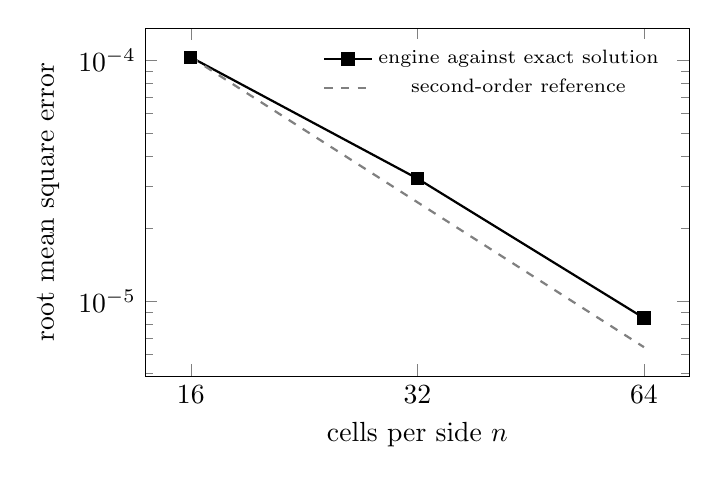
\begin{tikzpicture}
\begin{axis}[width=0.7\textwidth,height=6cm,xmode=log,ymode=log,xlabel={cells per side $n$},ylabel={root mean square error},
  xtick={16,32,64},xticklabels={16,32,64},
  legend style={at={(0.97,0.97)},anchor=north east,draw=none,font=\scriptsize,fill=white}]
\addplot[black,thick,mark=square*] coordinates {(16,1.03e-4) (32,3.23e-5) (64,8.51e-6)};
\addplot[gray,dashed,thick] coordinates {(16,1.03e-4) (32,2.575e-5) (64,6.44e-6)};
\legend{engine against exact solution,second-order reference}
\end{axis}
\end{tikzpicture}
% source: recomputed with privacy_risk.transport; tests/test_ext_transport.py
\caption{Error of the finite-volume solver against the exact diffusion solution \eqref{c20:eq-exact} at time
$0.2$ with dispersion $0.03$ and no drift. The measured errors (solid black line, filled squares) are set
beside a reference line falling with the square of the cell width (dashed grey line, drawn through the
first point). Synthetic benchmark; the measured slope steepens towards the reference as the grid is
refined.}
\label{c20:fig-refine}
\end{figure}

With the shear switched on at amplitude $0.2$ and smoothing $0.05$ on the $32\times32$ grid, the
engine took 33 steps with a stability number of $0.784$, the mass error was again zero and the
smallest value was $0.573$. These are the properties Proposition~\ref{c20:prop-stable} guarantees. There is no
exact solution for the density under shear with dispersion in the engine's tests, so the shear
run checks conservation and positivity, not accuracy.

Tom\'as's first runs were refused. He had asked for a coarse time step to save computing
time and, when the engine declined, asked Naledi whether the negative values could simply
be set to zero. She showed him Proposition~\ref{c20:prop-stable} and asked him to let the engine choose the
step. The runs that followed conserved mass to the last digit. Tom\'as took this as evidence
that the model was sound; Naledi took it as evidence that the solver was, and said the two
claims needed separate support.

\section{Bayesian inference over a finite prior}

A solver turns parameters into a forecast. The parameters themselves, the dispersion $D_c$ and
the drift amplitude $A$ in the simplest case, must come from data. Write $G_\eta$ for the map from
a parameter vector $\eta$ to predicted densities at the observation points and times, and $H$ for
the observation operator that selects them. A model for continuous observations is
\begin{equation}\label{c20:eq-obs}
y=HG_\eta+\delta+\varepsilon,\qquad\varepsilon\sim N(0,\Sigma),
\end{equation}
where $\delta$ is the discrepancy between the proposed dynamics and the world, the term that
\citet{kennedy2001} introduced for the calibration of computer models. Leaving
$\delta$ out forces every systematic error into the coefficients, which then look precisely estimated
and mean little. Putting it in creates its own identifiability problem, since a flexible discrepancy can absorb anything, and its prior has to be argued for; \citet{brynjarsdottir2014}
show that physical parameters are learned correctly only when that prior carries real
knowledge of the discrepancy. \citet{stuart2010} develops the Bayesian treatment of such
inverse problems in general; the disclosure application, and the feature geometry it needs,
remain proposals here.

Bayes' rule gives the posterior $p(\eta\mid y)\propto p(y\mid\eta)p(\eta)$. The engine computes it exactly
for a finite prior. If the prior puts weight $p_g$ on each of $G$ parameter vectors $\eta_g$ and $\ell_g=-\tfrac12\|y-HG_{\eta_g}\|^2_{\Sigma^{-1}}$ is the log likelihood, then
\begin{equation}\label{c20:eq-post}
w_g=\frac{\exp(\ell_g-\ell_{\max})\,p_g}{\sum_{h=1}^{G}\exp(\ell_h-\ell_{\max})\,p_h}.
\end{equation}
Subtracting the largest log likelihood $\ell_{\max}$ changes nothing in exact arithmetic and keeps
the exponentials from underflowing. The calculation is transparent: every weight can be
printed and checked. It is not a sampler for a continuous posterior, and it should be read as
one only after the grid has been refined and the prior range varied.

A forecast from the posterior must carry the posterior's uncertainty. If a future audit of
$B$ fresh targets yields $K$ successes, and given $\eta$ these are Binomial$(B,r_a(\eta))$, then the forecast
of $K$ is the mixture
\begin{equation}\label{c20:eq-mix}
\Prob(K=k\mid y)=\sum_{g=1}^{G}w_g\binom Bk r_a(\eta_g)^k\big(1-r_a(\eta_g)\big)^{B-k}.
\end{equation}
It is tempting to replace this by a single binomial at the posterior mean risk $\bar r=\sum_gw_gr_a(\eta_g)$.
That shortcut understates the spread.

\begin{proposition}[The predictive mixture is wider]\label{c20:prop-mix}
Let $K$ have the mixture law \eqref{c20:eq-mix} and let $\bar r$ be the posterior mean risk. Then
\[\mathrm{Var}(K\mid y)=B\bar r(1-\bar r)+B(B-1)\,\mathrm{Var}\big(r_a(\eta)\mid y\big)\ \ge\ B\bar r(1-\bar r),\]
with equality only when $B=1$ or the posterior puts all its weight on parameter vectors with the
same risk.
\end{proposition}

The extra term grows with the square of the audit size. For the audit sizes of Chapter~\ref{ch:estimate},
hundreds of attempts, even modest uncertainty in the risk dominates the binomial term, and
a plug-in forecast would describe the next audit as far more predictable than it is. This is the
same distinction Chapter~\ref{ch:learning} draws between planning figures and certificates: the mixture is
a planning figure, and no posterior, however it is computed, replaces the audit bound in the
release rule.

\begin{example}[Planning an audit of 400 attacks]\label{c20:ex-plan}
Suppose Tom\'as's posterior puts weight one
half on a risk of $0.05$ and one half on $0.10$, and Naledi plans an audit of 400 fresh attacks. The
numbers are illustrative. The posterior mean risk is $0.075$, and a single binomial at that risk
has mean 30, variance $400\times0.075\times0.925=27.75$ and standard deviation $5.3$. The posterior
variance of the risk is $0.025^2=0.000625$, so Proposition~\ref{c20:prop-mix} adds $400\times399\times0.000625=99.75$ to the variance, which becomes $127.5$, a standard deviation of $11.3$. The plug-in forecast
puts 95 per cent of the count between 20 and 41; the mixture puts it between 13 and 50. A
count of 40 or more has probability $0.04$ under the plug-in and $0.26$ under the mixture. A
plan sized on the plug-in would treat one audit in four as a surprise.
\end{example}

\section{What the evidence run recovered}\label{c20:sec-recovered}

The evidence run put a finite prior on 81 pairs $(D_c,A)$: nine dispersions equally spaced from
$0.01$ to $0.05$ and nine amplitudes from $0.1$ to $0.3$. It generated noisy observations at sixteen
points of a $16\times16$ grid at time $0.2$, from a true pair of $D_c=0.03$ and $A=0.2$, with noise of
standard deviation $0.01$, and computed the posterior \eqref{c20:eq-post}.

In the first case the observations were generated by the same solver, on the same grid,
that the inference used. In the extension's run the posterior mean was $0.0306$ for dispersion and $0.175$ for amplitude, with standard deviations of $0.0017$ and $0.020$, and the most probable pair was
$(0.03,0.175)$, with weight $0.44$. Dispersion was recovered to within a fraction of its grid
spacing. Amplitude was not: the most probable value sat one grid step below the truth, and
the truth lay about one and a quarter standard deviations above the mean. With one draw
of the noise this is not an error in the method. It is what a wide posterior looks like when
a single realisation is reported, and it is the first sign that the observations say much less
about the drift than about the dispersion.

The draw can be repeated. With the repository's solver, a lattice of 16 cell centres and three noise seeds, the posterior standard deviation of the amplitude came out at $0.019$ to $0.020$ and that of the dispersion at $0.0003$ to $0.0009$; the posterior mean of the amplitude was $0.222$, $0.245$ and $0.197$, and the most probable amplitude was $0.225$, $0.25$ and $0.2$. These runs used the repository's code and differ from the extension's draw, so the individual means are different and the spread is the same. One draw can land on either side of the truth, and the spread is the stable result.

In the second case the observations came from a finer, $32\times32$ solver run with the same
true parameters, sampled at sixteen points, while the inference still used the $16\times16$ model.
In the extension's run the posterior mean was $0.0300$ for dispersion and $0.193$ for amplitude, the most probable
pair was the truth, $(0.03,0.2)$, with weight $0.49$, and the standard deviations were $0.00035$
and $0.019$. The mismatched case landed closer to the truth than the matched one. Read
naively, that would say that model error helps. Two features of the run warn against the
reading. The noise draws differ between the two cases, and with one draw each, which case
lands closer is partly luck. And the dispersion standard deviation of $0.00035$ is smaller than
the prior's grid spacing of $0.005$: almost all the weight sits on one dispersion value, so the
reported spread measures the coarseness of the prior, not the information in the data. A
narrow posterior produced by a coarse or strong prior is not identification.

Tom\'as brought the first posterior to Naledi as a success: the dispersion had come back
almost exactly. She agreed, and asked about the drift. His model's central claim was that
drift could be forecast, and the drift was the parameter the data had resolved least well. She
asked him for the spectrum that the engine reports beside every posterior.

\begin{figure}[ht]
\centering
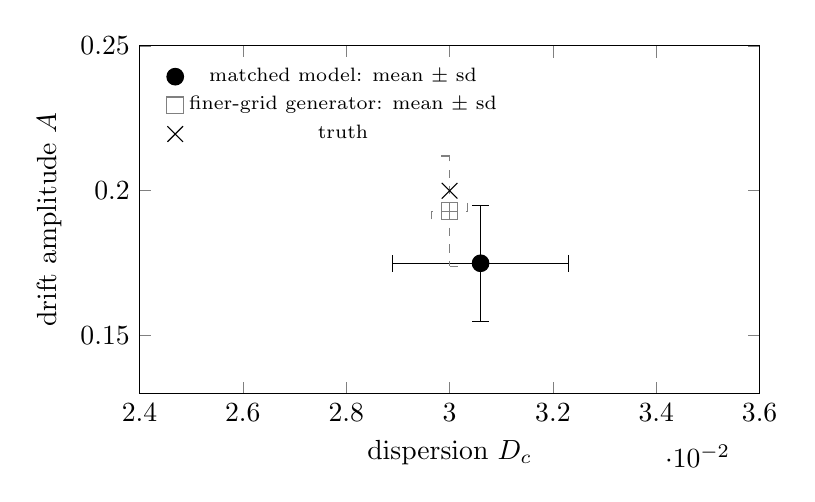
\begin{tikzpicture}
\begin{axis}[width=0.78\textwidth,height=6cm,xlabel={dispersion $D_c$},ylabel={drift amplitude $A$},
  xmin=0.024,xmax=0.036,ymin=0.13,ymax=0.25,
  legend style={at={(0.03,0.97)},anchor=north west,draw=none,font=\scriptsize,fill=white}]
\addplot[black,only marks,mark=*,mark size=3pt,error bars/.cd,x dir=both,x explicit,y dir=both,y explicit]
  coordinates {(0.0306,0.175) +- (0.0017,0.020)};
\addplot[gray,only marks,mark=square,mark size=3pt,error bars/.cd,x dir=both,x explicit,y dir=both,y explicit,error bar style={dashed}]
  coordinates {(0.0300,0.193) +- (0.00035,0.019)};
\addplot[black,only marks,mark=x,mark size=4pt] coordinates {(0.03,0.2)};
\legend{matched model: mean $\pm$ sd,finer-grid generator: mean $\pm$ sd,truth}
\end{axis}
\end{tikzpicture}
% source: draft 2 text of Section 20.7 (the extension's run)
\caption{Posterior means and standard deviations for dispersion and drift amplitude under the
81-point finite prior, from the extension's run, shown near the truth. The matched-model posterior (filled black circle, solid bars) and the finer-grid posterior (open grey square, dashed
bars) are told apart by mark, shade and bar style; the cross marks the truth. Synthetic observations.}
\label{c20:fig-post}
\end{figure}

\section{Identifiability and the singular values}

Whether data can resolve a parameter is a property of the forward model and the observation design, and it can be checked before any posterior is computed. Let $J$ be the Jacobian of the predicted observations with respect to the parameters, the matrix of sensitivities
$J_{ih}=\partial(HG_\eta)_i/\partial\eta_h$. Its singular values measure how strongly the observations respond to
movement along each direction in parameter space. A large singular value marks a direction the data resolve; a small one marks a direction the data barely see. Under the Gaussian
model \eqref{c20:eq-obs} with $\Sigma=\sigma^2I$ and no discrepancy, the Fisher information is $J^\top J/\sigma^2$, and near
the truth the posterior standard deviation along a direction with singular value $s$ is about
$\sigma/s$.

At the true pair the engine's finite-difference Jacobian had singular values of $7.13$ and
$0.515$, a condition number of $13.8$. The Fisher information had eigenvalues of about $508{,}000$
and $2{,}650$. With $\sigma=0.01$ these give standard deviations of about $0.0014$ and $0.019$ along
the two directions. The second figure matches the amplitude's posterior standard deviation
of $0.020$ in the matched case, which says that the weak direction is the amplitude. The
observations at one time respond to the dispersion through the overall decay of the pattern,
which is large and easy to see; they respond to the drift only through a small sideways shift
of it. The repository's \texttt{bayes.sensitivity\_spectrum}, on a lattice of 16 cell centres, gives $7.09$ and $0.516$, a condition number of $13.7$, and Fisher eigenvalues of about $502{,}700$ and $2{,}660$.
The small difference from the extension's figures comes from where the sixteen observation points sit, which the extension does not state.

A condition number of fourteen is mild. Models in systems biology commonly show
sensitivity spectra spread over many orders of magnitude \citep{gutenkunst2007}. A model
with a full drift field, a forcing term, an initial condition and an attack response, fitted to one
scalar risk series, would have many more directions and far smaller singular values in most
of them. One risk series cannot normally identify a two-dimensional velocity field. The
order of work this implies is plain: fix the attack response and the initial condition, estimate
a few coefficients, report the spectrum, and add parameters only while the spectrum shows
that the data can carry them.

\section{The inverse crime}

The matched case of Section~\ref{c20:sec-recovered}'s first run generated its data with the same model, the same grid
and the same observation operator that the inference then assumed. In the literature on inverse
problems this is called an inverse crime \citep{kaipio2007}. It makes recovery
look easier than it is, because every error the model makes when generating is made again,
identically, when inferring, and the two cancel. A matched-model run is a pipeline check:
it shows that the code computes the posterior it was written to compute. It is not external
validation, and the engine's documentation says so beside the function. The finer-grid case
is one step away from the crime. It changes the mesh, and with it the positions of the sixteen
observation points, which in the finer grid sit half a coarse cell away from where the coarse
model expects them. It does not change the model family, the noise law or the drift. A real
validation would generate observations independently of the model, perturb the dynamics
and the observation operator, and include data the model was not designed for, which for a
register means data from vintages held out of every fitting step.

Tom\'as had committed the crime in his first draft without knowing its name. His synthetic register had been made by his own solver, and his recovery of the drift from it was
the result his note led with. Naledi asked him to move it to an appendix headed as a check
of the code, and to leave the main text for data his solver had not made.

\section{A PDE surrogate is a separate task}

When a solver is slow, a common next step is to train a neural network to approximate
it. A physics-informed network outputs fields $(u_\phi,\pi_\phi,c_\phi)$ and is trained to fit observations
while keeping the residuals of \eqref{c20:eq-ad}, \eqref{c20:eq-ns} and \eqref{c20:eq-div} small at chosen collocation points
\citep{raissi2019}. Such a surrogate answers a different question from the risk planner
of Chapter~\ref{ch:planner}. The planner predicts attack success from measured counts; the surrogate
approximates a solver. Mixing the two would let a network trained on its own simulated
output stand in for evidence about attacks.

Surrogates also fail in documented ways. A small residual at the training points need
not mean a small error between them, and optimisation can stall on solutions that satisfy the
equations poorly \citep{krishnapriyan2021}. A surrogate must therefore be compared with
an independent solver on held-out parameter settings and time windows, and checked for
mass and positivity, which a network does not respect by construction. Here the equation
is itself a proposed model of how borrowers move, so the name physics-informed should
not be read as physical validation of anything about disclosure. The engine does not train
a surrogate, and the extension plans one only if the cost of the finite-volume solver ever
justifies it.

\section{The baseline the transport model must beat}\label{c20:sec-baseline}

Every model in this chapter has a simpler competitor. Many of the movements Tom\'as
wanted to forecast are between categories: a borrower moves from one lender to another,
from one size class to the next, from performing to non-performing. A continuous-time
Markov chain on a graph of such states describes these moves without any geometry, and
credit-risk work has long used it for movements between rating grades \citep{jarrow1997}.
If $c_i(t)$ is the mass at node $i$ and $Q$ is a generator, with nonnegative rates $Q_{ij}$ off the diagonal
and rows summing to zero, then
\[\dot c=Q^\top c,\qquad c(t)=\exp(tQ^\top)\,c(0),\]
and node risks $g_i$ give the model risk $r=g^\top c/\mathbf 1^\top c$, the graph version of \eqref{c20:eq-risk}. The nonnegative rates keep masses nonnegative and the zero row sums keep total mass constant, the
same two properties Proposition~\ref{c20:prop-stable} proves for the transport solver. Chapter~\ref{ch:change} develops
this baseline and its estimation from observed transitions. In the evidence run the engine
recovered a four-node generator from 400 simulated paths with a largest rate error of $0.016$,
and the propagated masses still summed to one.

Figure~\ref{c20:fig-ladder} sets out the order of comparison the extension specifies. Each model on the
ladder adds assumptions to the one before. A model earns its place only by forecasting
held-out periods better than the model below it, or by carrying a structural constraint that
is independently known to hold.

\begin{figure}[ht]
\centering
\begin{tikzpicture}[>=stealth,built/.style={draw,fill=gray!20,minimum width=2.3cm,minimum height=1.1cm,align=center,font=\small},
  notbuilt/.style={draw,dashed,pattern=north east lines,pattern color=gray!60,minimum width=2.3cm,minimum height=1.1cm,align=center,font=\small,fill=white}]
\node[built] (a) at (0,0) {static\\ hierarchical};
\node[built] (b) at (2.9,0) {exposure and\\ activity};
\node[built] (c) at (5.8,0) {graph\\ generator};
\node[built] (d) at (8.7,0) {scalar transport,\\ exact shear};
\node[notbuilt,fill=white] (e) at (11.6,0) {\colorbox{white}{general}\\ \colorbox{white}{Navier--Stokes}};
\draw[->] (a)--(b); \draw[->] (b)--(c); \draw[->] (c)--(d); \draw[->] (d)--(e);
\node[font=\scriptsize,align=center] at (5.8,-1.3) {each step must forecast held-out periods better than the step before it:\\ comparison not yet run on any rung};
\end{tikzpicture}
\caption{The ladder of dynamic models, from fewest assumptions (left) to most (right). Models
built and tested in the engine have solid borders and grey fill; the general Navier--Stokes solver, not
built, has a dashed border and hatching. The arrows mark the comparisons the extension requires;
none has been run on held-out data.}
\label{c20:fig-ladder}
\end{figure}

The comparison has not been run on any rung. The engine has the static model of the
earlier chapters, the exposure and activity panel, the graph generator and the scalar transport solver under an exact shear, each with tests of its own properties. It has no experiment
in which any of them forecasts held-out vintages of a register and is scored against another.
Until that experiment exists, nothing in this book supports the claim that a transport model,
with or without the Navier--Stokes closure, forecasts disclosure risk better than a table of
counts.

The committee met to consider Tom\'as's proposal with Figure~\ref{c20:fig-ladder} on the table. The chair
asked which rung the proposal sat on, and Naledi pointed to the last one. The committee
recorded the model as research, approved Tom\'as's use of synthetic data to run the comparison against the graph baseline, and stated that no forecast from it would enter a release
decision until it had beaten that baseline on held-out vintages. Grace, reading the record
later, found the condition written in a form she could check.

\section{The answer}

The chapter asked what a dynamic model of the target population would have to show before its forecast could enter a release decision. It has to show five things, and each has a test.
Its density must obey a stated balance law, and its solver must preserve mass and positivity
without clipping, which Proposition~\ref{c20:prop-stable} guarantees under a bound the engine enforces. Its
link to disclosure must run through an attack response fitted to measured outcomes, as in
\eqref{c20:eq-risk}. Its parameters must be identified by the data, shown by the singular values of the
sensitivity matrix and not by the narrowness of a posterior on a coarse grid. Its validation
must use data that the model did not generate. And it must forecast held-out periods better
than the graph baseline and the simpler models below it. The engine meets the first and
supplies the tools for the second and third. The fourth and fifth have not been done. A
model drawn from physics brings structure, and structure is a set of assumptions; until the
comparison is run, the Bank's release decisions rest on audits of attacks, as the rest of this
book describes.

\begin{inpractice}[In practice: a proposal for a dynamic risk model]
Ask the proposer to name, in the register's own terms, the feature space, the density and
the attack response, and to state where the response was fitted. Ask for the balance law and
for the treatment of entry and exit. Require a solver check against an exact solution, with mass
and minimum reported at every run, and refuse any solver that clips. Require the identifiability
spectrum beside every posterior, and treat a matched-model recovery as a pipeline check only.
Record the model's place on the ladder of Figure~\ref{c20:fig-ladder} and the held-out comparison it must win
before any forecast enters a decision record. Until then, record it as research.

\medskip\noindent\textit{In the software.} The solver, the exact diffusion solution and the model risk integral are in
\texttt{privacy\_risk.transport} (\texttt{transport}, \texttt{exact\_diffusion}, \texttt{risk\_from\_density}; the last uses
a declared toy response unless a fitted one is passed). The finite-prior posterior, the
transport forward model, the predictive mixture and the spectrum are in \texttt{privacy\_risk.bayes} (\texttt{grid\_posterior},
\texttt{transport\_forward}, \texttt{predictive\_pmf}, \texttt{sensitivity\_spectrum}). The graph baseline is in \texttt{privacy\_risk.graph}.
The tests in \texttt{tests/test\_ext\_transport.py} check mass, positivity, refinement, refusal of unstable steps, normalisation of the posterior, Example~\ref{c20:ex-plan} and the spectrum. Algorithm~20.1 sets out one run of the solver with its stability check, and its checks replay Example~\ref{c20:ex-step} and the refinement study of Figure~\ref{c20:fig-refine}.
\end{inpractice}

\begin{mdframed}[linecolor=gray!60,backgroundcolor=gray!5]
\textbf{Algorithm 20.1.} One run of the transport solver.\par\smallskip
\textit{Input.} A grid of $n\times n$ cells; a horizon $T$; a dispersion $D_c$; a drift amplitude $A$ and smoothing $\nu$;
an initial density $c_0$ (by default \eqref{c20:eq-exact} at $t=0$, sampled at cell centres); and, optionally, a number
of steps $M$.\par
\textit{Output.} The density $c_M$ at time $T$, with its mass error, its smallest value, the number of steps, the
step $\Delta t$ and the stability number.
\begin{enumerate}
\item Refuse the inputs unless $n$ is a whole number of at least 8, $T$, $D_c$, $A$ and $\nu$ are finite, and $T$,
$D_c$ and $\nu$ are not negative. Refuse an initial density that is not $n\times n$, finite and nonnegative.
\item Set $h=1/n$ and the rate bound $R=|A|/h+4D_c/h^2$, the bracket of \eqref{c20:eq-cfl}.
\item If $M$ is not given, take the least $M\ge1$ with $TR/M\le0.8$. If it is given, refuse $M<1$.
\item Set $\Delta t=T/M$. If $\Delta t\,R>0.8$, refuse the request and report the stability number $\Delta t\,R$; never clip.
\item For $m=0,1,\dots,M-1$: set the drift in row $j$ to $u_j=Ae^{-\nu(2\pi)^2m\Delta t}\sin(2\pi y_j)$, from \eqref{c20:eq-shear},
with $y_j$ the height of the row's centre, and update every cell by \eqref{c20:eq-update}, with indices taken
modulo $n$.
\item Return $c_M$, the mass error $\bar c_M-\bar c_0$ where the bar is the mean over cells, $\min c_M$, $M$, $\Delta t$ and
$\Delta t\,R$. By Proposition~\ref{c20:prop-stable} the mass error is zero up to rounding and the minimum does not
fall.
\end{enumerate}
\textit{Checks, each run against the software by the test suite:}
\begin{itemize}
\item One step of $\Delta t=0.0667$ from all the mass in one cell at height $0.3125$ on an $8\times8$ grid, with
$D_c=0.03$, $A=0.2$, $\nu=0.05$ (Example~\ref{c20:ex-step}), share the cell keeps: $0.3891$.
\item The same, share of the cell downstream: $0.2267$.
\item The same, share of the cell upstream: $0.1281$.
\item The same, stability number: $0.619$.
\item No drift, a $32\times32$ grid, horizon $0.2$ and $D_c=0.03$, steps left to the solver, number of steps: 31.
\item The same, stability number: $0.793$.
\item The same, mass error: $0.0000$.
\item A horizon of zero, number of steps: 1.
\item One step of $\Delta t=0.2$ from the single cell of Example~\ref{c20:ex-step}, stability number $1.856$: refused.
\item Two steps over a horizon of $0.2$ on a $32\times32$ grid with $A=0.2$ and $D_c=0.03$, as in the evidence run: refused.
\item A grid of 4 cells a side: refused.
\end{itemize}
\end{mdframed}

\section{Proofs}

\begin{proof}[Proof of Proposition~\ref{c20:prop-energy}]
Take the inner product of \eqref{c20:eq-ns} with $u$ and integrate over the periodic domain. The time derivative gives $\int u\cdot\partial_tu\,dx=\tfrac12\tfrac d{dt}\|u\|_2^2$. For the nonlinear term,
$u\cdot(u\cdot\nabla)u=\sum_ju_j\partial_j|u|^2/2$, and integration by parts on the periodic domain, where
boundary terms vanish, gives $\int u\cdot(u\cdot\nabla)u\,dx=-\int(\nabla\cdot u)|u|^2/2\,dx=0$ by \eqref{c20:eq-div}. In the
same way $\int u\cdot\nabla\pi\,dx=-\int\pi\nabla\cdot u\,dx=0$. For the smoothing term, integration by parts
in each component gives $\nu\int u\cdot\Delta u\,dx=-\nu\sum_{i,j}\int(\partial_ju_i)^2dx=-\nu\|\nabla u\|_2^2$. The forcing gives
$\langle f,u\rangle$. Collecting terms yields \eqref{c20:eq-energy}.
\end{proof}

\begin{proof}[Proof of Proposition~\ref{c20:prop-exact}]
For part 1, write $u_1=Ae^{-\nu k^2t}\sin(ky)$ and $u_2=0$. Then $\nabla\cdot u=\partial_xu_1=0$, since $u_1$ does not depend on $x$, so \eqref{c20:eq-div} holds. The convective term is $(u\cdot\nabla)u=u_1\partial_xu=0$. The time derivative is $\partial_tu_1=-\nu k^2u_1$ and the Laplacian is $\Delta u_1=\partial_{yy}u_1=-k^2u_1$,
so $\partial_tu_1=\nu\Delta u_1$. With $\pi=0$ and $f=0$ both components of \eqref{c20:eq-ns} hold. For the energy
identity, the mean of $\sin^2(ky)$ over the unit square is $\tfrac12$, so $\|u\|_2^2=\tfrac12A^2e^{-2\nu k^2t}$ and $\tfrac12\tfrac d{dt}\|u\|_2^2=-\tfrac12\nu k^2A^2e^{-2\nu k^2t}$; and $\|\nabla u\|_2^2=\|\partial_yu_1\|_2^2=\tfrac12k^2A^2e^{-2\nu k^2t}$. The two sides of \eqref{c20:eq-energy} then sum to
zero, which is $\langle f,u\rangle$.

For part 2, with $u=0$ and $s=0$ the equation is $\partial_tc=D_c\Delta c$. Each of $\cos(kx)$ and $\sin(ky)$
is an eigenfunction of the Laplacian with eigenvalue $-k^2$, so $e^{-D_ck^2t}$ times either solves the
equation, as does the constant 1; by linearity so does \eqref{c20:eq-exact}. The two trigonometric terms
have mean zero over the unit square, so the mass is one. Finally $c\ge1-e^{-D_ck^2t}(0.35+0.20)\ge1-0.55>0$.
\end{proof}

\begin{proof}[Proof of Proposition~\ref{c20:prop-stable}]
Fix a row $j$ and write $a=\Delta t/h$, $d=D_c\Delta t/h^2$, $u=u_j$. Substituting the fluxes into \eqref{c20:eq-update},
\[c^{m+1}_{i,j}=c_{i,j}-a\big(u^+c_{i,j}+u^-c_{i+1,j}-u^+c_{i-1,j}-u^-c_{i,j}\big)+d\big(c_{i+1,j}+c_{i-1,j}+c_{i,j+1}+c_{i,j-1}-4c_{i,j}\big),\]
where all values on the right are at step $m$. Since $u^+-u^-=|u|$, collecting terms gives
\[c^{m+1}_{i,j}=\big(1-a|u|-4d\big)c_{i,j}+\big(au^++d\big)c_{i-1,j}+\big(d-au^-\big)c_{i+1,j}+d\,c_{i,j+1}+d\,c_{i,j-1}.\]
The last four weights are nonnegative because $u^+\ge0$, $u^-\le0$ and $d\ge0$. The first is at least
$1-\Delta t(|A|/h+4D_c/h^2)\ge0.2$ by $|u|\le|A|$ and \eqref{c20:eq-cfl}. The weights sum to $1-a|u|-4d+au^+-au^-+4d=1$. So $c^{m+1}_{i,j}$ is a weighted average of five values at step $m$, and it is at least
their minimum; hence $\min c^{m+1}\ge\min c^m$, and nonnegativity follows by induction.

For mass, sum \eqref{c20:eq-update} over all cells. Within each row the flux differences $F_{i+1/2,j}-F_{i-1/2,j}$
telescope to zero around the periodic index $i$. The diffusion term sums to $\sum_{i,j}(c_{i+1,j}+c_{i-1,j}+c_{i,j+1}+c_{i,j-1})-4\sum_{i,j}c_{i,j}=0$, because each shifted sum runs over all cells once. Hence
$\sum_{i,j}c^{m+1}_{i,j}=\sum_{i,j}c^m_{i,j}$.
\end{proof}

\begin{proof}[Proof of Proposition~\ref{c20:prop-mix}]
Write $R=r_a(\eta)$ with $\eta$ drawn from the posterior, so that $K\mid R$ is
Binomial$(B,R)$. By the law of total variance,
\[\mathrm{Var}(K)=\E[\mathrm{Var}(K\mid R)]+\mathrm{Var}(\E[K\mid R])=\E[BR(1-R)]+\mathrm{Var}(BR).\]
The first term is $B\bar r-B\,\E[R^2]=B\bar r-B(\mathrm{Var}\,R+\bar r^2)=B\bar r(1-\bar r)-B\,\mathrm{Var}\,R$, and the second
is $B^2\mathrm{Var}\,R$. Their sum is $B\bar r(1-\bar r)+B(B-1)\mathrm{Var}\,R$. The added term is nonnegative, and
it is zero exactly when $B=1$ or $\mathrm{Var}\,R=0$, that is, when $R$ takes one value with posterior
probability one.
\end{proof}
